%!TEX root = ../thesis.tex
\begin{savequote}[75mm]
Nulla facilisi. In vel sem. Morbi id urna in diam dignissim feugiat. Proin molestie tortor eu velit. Aliquam erat volutpat. Nullam ultrices, diam tempus vulputate egestas, eros pede varius leo.
\qauthor{Quoteauthor Lastname}
\end{savequote}

\chapter{Discussion}
\label{chap:discussion}

\newthought{The results of the experiments} detailed in Chapter \ref{chap:results} suggest a few relationships between the Discrete Voter Model (DVM) and King's Ecological Inference method (KEI):

\begin{enumerate}
  \item In the $2 \times 2$ case, DVM runs as quickly as KEI for the same number of steps, using Random Walk Metropolis (RWM) as the kernel and expectation-based scoring. It is slower with the Hamiltonian Monte Carlo kernel and either scoring function, and with RWM and probability-based scoring.
  \item In the $2 \times 2$ case, KEI is more accurate than DVM in nearly all elections, but the results are close.
  \item Unlike KEI, DVM can produce reliable results for the $3 \times 2$ case (three demographic groups and two candidates) in a reasonable amount of time.
\end{enumerate}

The results also suggest a few relationships among the DVM configurations. Each of the following relationships is observed in the context of controlling for other variables (ceteris paribus: with other conditions remaining the same).

\begin{enumerate}
  \item The Random Walk Metropolis (RWM) kernel is faster than the Hamiltonian Monte Carlo (HMC) kernel.
  \item The HMC kernel produces more accurate results than the RWM kernel.
  \item Expectation-based scoring is faster than probability-based scoring.
  \item Expectation-based scoring is often just as accurate, if not more accurate, than probability-based scoring.
  \item Higher granularity probability hypercubes cause DVM to take more time.
  \item When the chain is run for longer, DVM produces more accurate results.
\end{enumerate}

There are many variables contributing to the results of these experiments in more specific ways than the relationships and trends noted above. Section \ref{sec:params} discusses their effects.

\section{The Effect of DVM's Parameters}
\label{sec:params}

\subsection{PHC Granularity}

\newthought{The results show} that the higher the granularity of the probabilistic hypercubes in the model, the slower the model but the more accurate the results.

Figure \ref{fig:1_1_mean_mse} shows that the MSE of the high-granularity PHC is less than half that of the lower-granularity PHC when scoring by either expectation or probability. Figure \ref{fig:1_1_time} shows that this configuration is the most time-intensive of all configurations with the same kernel and scoring function. Similar trends can be observed in the other elections, illustrated in Tables \ref{table:rwm_expec_2d} to \ref{table:hmc_2d} and Figures \ref{fig:1_1_time_append} to \ref{fig:3_2_mean_mse}.

With that said, the time-intensiveness of running DVM on such high granularity probability hypercubes made it infeasible to run DVM on elections with more than  $2$ demographic groups. However, having high granularity PHCs is not the only, and not the best, way to get accurate results in a reasonable time frame on a typical computer.

There is a clear tradeoff between time or computing power and accuracy if one chooses to vary the PHCs' granularities.

\subsection{Number of MCMC Steps}

\newthought{The results show} that the higher the number of steps in the Markov chain, the more accurate the model, and the slower the model.

Figure \ref{fig:1_1_mean_mse} shows that the MSE of the configuration with more steps was more accurate than the configuration with fewer steps when scoring by expectation. DVM in the configurations with a high number of steps and scored by probability are less accurate than than the lower number of steps and high granularity configurations in election $d_1 \times v_1$. However, in several other elections, like $d_1 \times v_2$ and $d_3 \times v_2$, illustrated in Figures \ref{fig:1_2_mean_mse} and \ref{fig:3_2_mean_mse} respectively, the configurations with the higher number of steps are more accurate.

Running the chain for more steps is necessarily more time-intensive than running it for fewer, but it is less time-intensive than running for fewer on high granularity PHCs.

Given that running the chain for more steps produces better results in a shorter amount of time than increasing the granularity of the PHCs, it is advisable to increase the number of steps in the chain to increase the accuracy of DVM, instead of increasing the granularity of the PHCs.

\subsection{Kernel}

\newthought{The results show} that the Hamiltonian Monte Carlo (HMC) kernel is more time-intensive, for the same number of steps, than the Random Walk Metropolis (RWM) kernel, but is generally more accurate.

For most elections in the $2 \times 2$ case, including $d_1 \times v_1$ illustrated in Figure \ref{fig:1_1_mean_mse}, HMC is more accurate than many of the other configurations. It is most comparable in accuracy to the similarly strong RWM kernel run for $10$ times more steps. When comparing the two on the same ``number of steps", however, HMC is more accurate.

This aligns with the research, intuition, and design of HMC. A ``step" in HMC is not the same as a ``step" in RWM. In the former, the ``step" is much more deliberate and intricate, doing several optimizations to move the chain in the direction of highest probability density. Hence, a $1$:$1$ comparison of HMC and RWM, on the basis of steps, is not useful. With that said, one can compare the amount of time that each needs to produce results with a certain amount of accuracy. HMC is consistently on par, if not a little faster, than RWM with a large number of steps. Nearly every figure in the range \ref{fig:1_1_mean_mse_append} to \ref{fig:3_2_mean_mse} shows this.

HMC also shines in the $3 \times 2$ case, consistently outperforming RWM when both are scored by expectation.

HMC and RWM are comparable when RWM is run for more steps, and when both are run for about the same amount of time. The tradeoff here is the same for deciding to run the chain for longer using RWM: HMC is typically more time- and compute-intensive, but it does produce good results. With that said, RWM's results are quite comparable, and if time or computing resources are strained, it should probably be preferred.

\subsection{Score Function}

\newthought{The results show} that scoring by probability is almost always more time-intensive than scoring by expectation, but does not usually produce more accurate results.

For about half of the elections analyzed, scoring by probability was worse than scoring by expectation. Figures \ref{fig:1_1_mle_mse} and \ref{fig:1_1_time} are good examples of this. Every expectation-based counterpart to the probability-based configuration was more accurate. The expectation-based configurations were also orders of magnitude faster than the probability-based configurations. The difference is even more stark with HMC configurations, where scoring by expectation was always more accurate than scoring by probability.

In the $3 \times 2$ case, like with configurations that increased the number of steps and granularity of the PHCs, scoring by probability was computationally infeasible on the typical computer, within a reasonable time frame.

Hence, scoring by expectation should almost always be preferred when using the Discrete Voter Model.


\subsection{The Recommended Configuration}

\newthought{Like most statistical models}, there is no perfect configuration of parameters that will work for all cases. The Discrete Voter Model is implemented such that switching between different configurations of parameters is simple, and that exploration is high encouraged.

With that said, the experiments conducted suggest that using the Random Walk Metropolis kernel, scoring by expectation, and running the model for a large number of steps on moderately-sized probability hypercubes generally produces better samples of the true distribution, and more accurate results.

That configuration was employed on the case studies from Chicago presented in Section {sec:chi}.


\section{Case Studies: Chicago 2015 and 2019 Mayoral Runoffs}
\label{sec:chicago}

\newthought{Chicago} is a large, beautiful and diverse city with a strong political system and culture of civic participation. Chicago also suffers from well-known problems in its electoral and civic structures, including gentrification, racial segregation, and gerrymandering.

The Metric Geometry and Gerrymandering Group (MGGG) notes in their \textit{Study of Reform Proposals for Chicago City Council}:

\begin{quote}
 The wards are perceived to be gerrymandered, with eccentric boundaries that preserve some traditionally favored neighborhoods but wind awkwardly through other parts of the city, denying Austin and Little Village the political stability that Bridgeport and Beverly have enjoyed for years. They also tend toward extreme malapportionment by the end of their ten-year cycle, with the largest ward having twice the population of the smallest, flouting the Constitutionally recognized principle of ``One Person, One Vote." Further, we will demonstrate that the current wards are massively racially segregated, far beyond the levels that would be expected in a 50-ward plan, and exhibit high levels of economic stratification as well. And legacy policies like ``aldermanic privilege" combine with carefully chosen lines to entrench some aldermen beyond the reach of accountability to their voters, creating what some have described as a system of fifty fiefdoms.\cite{chi_report}
\end{quote}

This damning assessment of Chicago's electoral system, and particularly the suspected gerrymandering of its wards, makes it an excellent case study for the Discrete Voter Model.

\begin{figure}[ht]\centering
 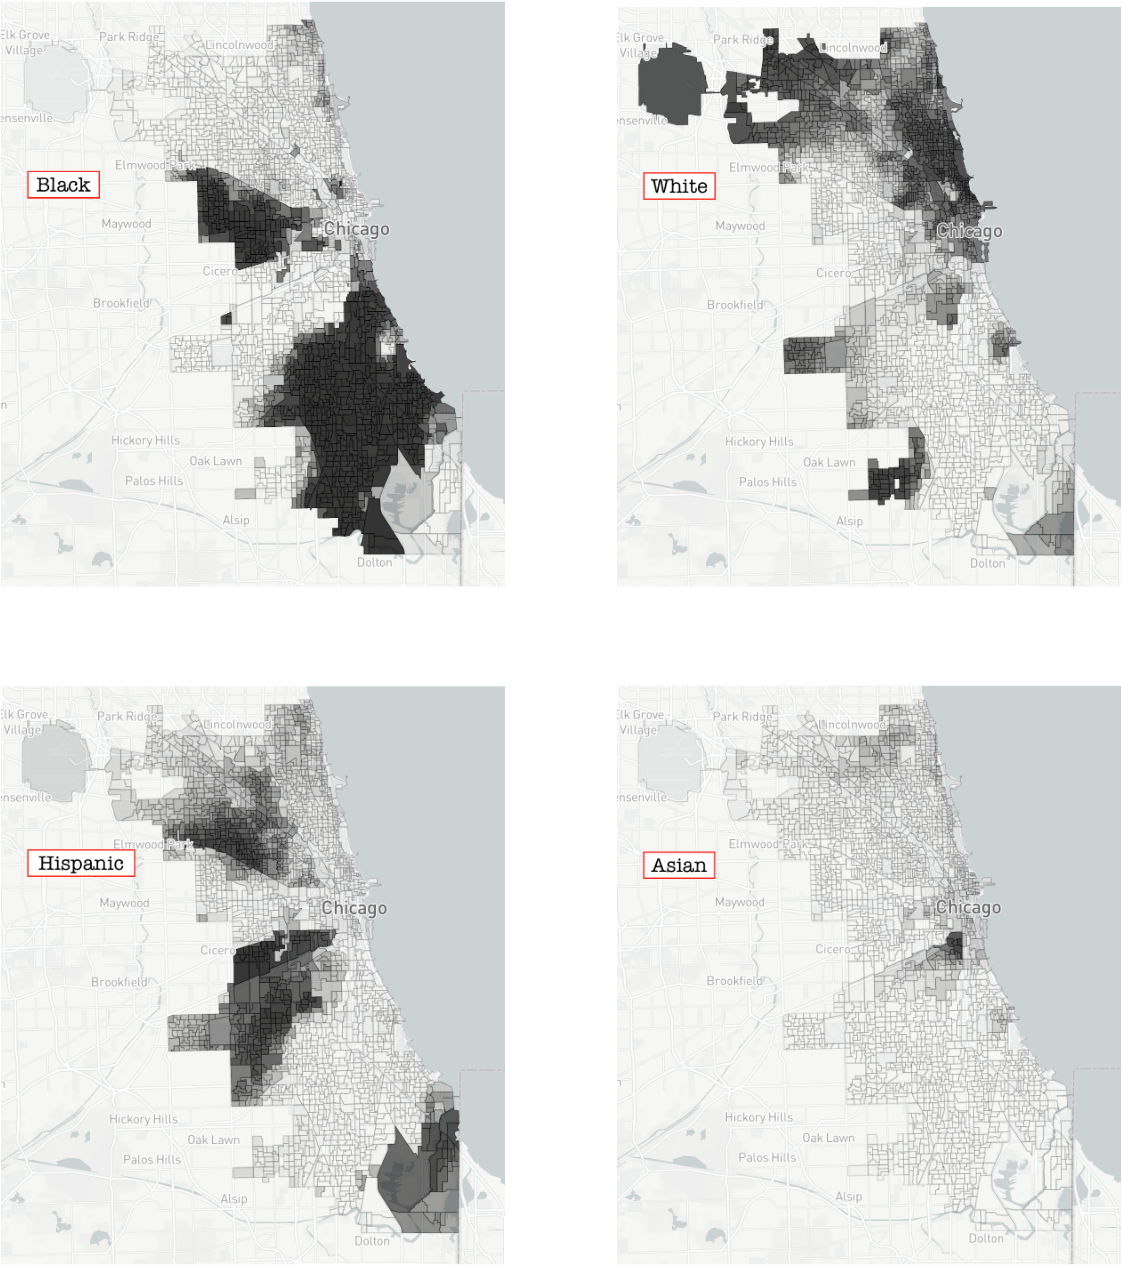
\includegraphics[width=\linewidth]{figures/chi_chloropleth.png}
 \caption{Choropleth Maps of the Four Largest Racial Groups in Chicago. Figure $2$ in MGGG's Chicago Report.\cite{chi_report}}
 \label{fig:chi_chloropleth}
\end{figure}

Of the $2069$ voting precincts in Chicago, $563$ are more than $90\%$ Black while $1054$ have less than $10\%$ Black population.\cite{chi_report}. To help visualize the dramatic racial segregation, Figure \ref{fig:chi_chloropleth} shows the chloropleth maps of the four largest racial groups in Chicago. Similar patterns exist along other axes of identity, like socioeconomic status.

Chicago's diverse and politically active electorate has more than the $2$ demographic groups that previous methods of determining racially polarized voting would allow. That racial diversity, combined with the massive amounts of segregation, sets up the perfect storm for racial gerrymandering, and necessitates a method like the Discrete Voter Model. The Discrete Voter Model also does not need to use race as the category for its demographic groups. Models can be easily built along other separations of the electorate, like socioeconomic status and age, or combinations of them.

Two recent runoff Mayoral elections, between Rahm Emanuel and Jesús "Chuy" García in 2015, and Lori Lightfoot and Toni Preckwinkle in 2019, are analyzed in this case study, with race as the demographic groups of interest.

\FloatBarrier
\subsection{Data Gathering}

\newthought{Electoral and demographic data} for Chicago were generously provided by the \href{https://mggg.org/chicago}{Metric Geometry and Gerrymandering Group}, and is available publicly in a \href{https://github.com/mggg/chicago}{GitHub repository}.

The data were cleaned to extract the necessary fields for the Discrete Voter Model, namely the precinct IDs, ward IDs, demographic fields, and electoral outcome fields.

In order to facilitate visualization, the data presented here were also clipped to include the three racial groups with the highest populations, identified as they are in the Census: Black, white, and Hispanic Chicagoans. However, model was still successfully run on full versions of the electorate, which also included Asian and other Chicagoans.


\subsection{Results}

\newthought{The Discrete Voter Model} was applied to Chicago's 2015 and 2019 Mayoral runoff elections, with Black, white, and Hispanic voters as the demographic groups.

DVM was configured to run for $10000$ steps, with the Random Walk Metropolis kernel and expectation-based scoring on granularity $10$ probability hypercubes, with a burn-in fraction of $0.3$.

\begin{figure}[ht]\centering
 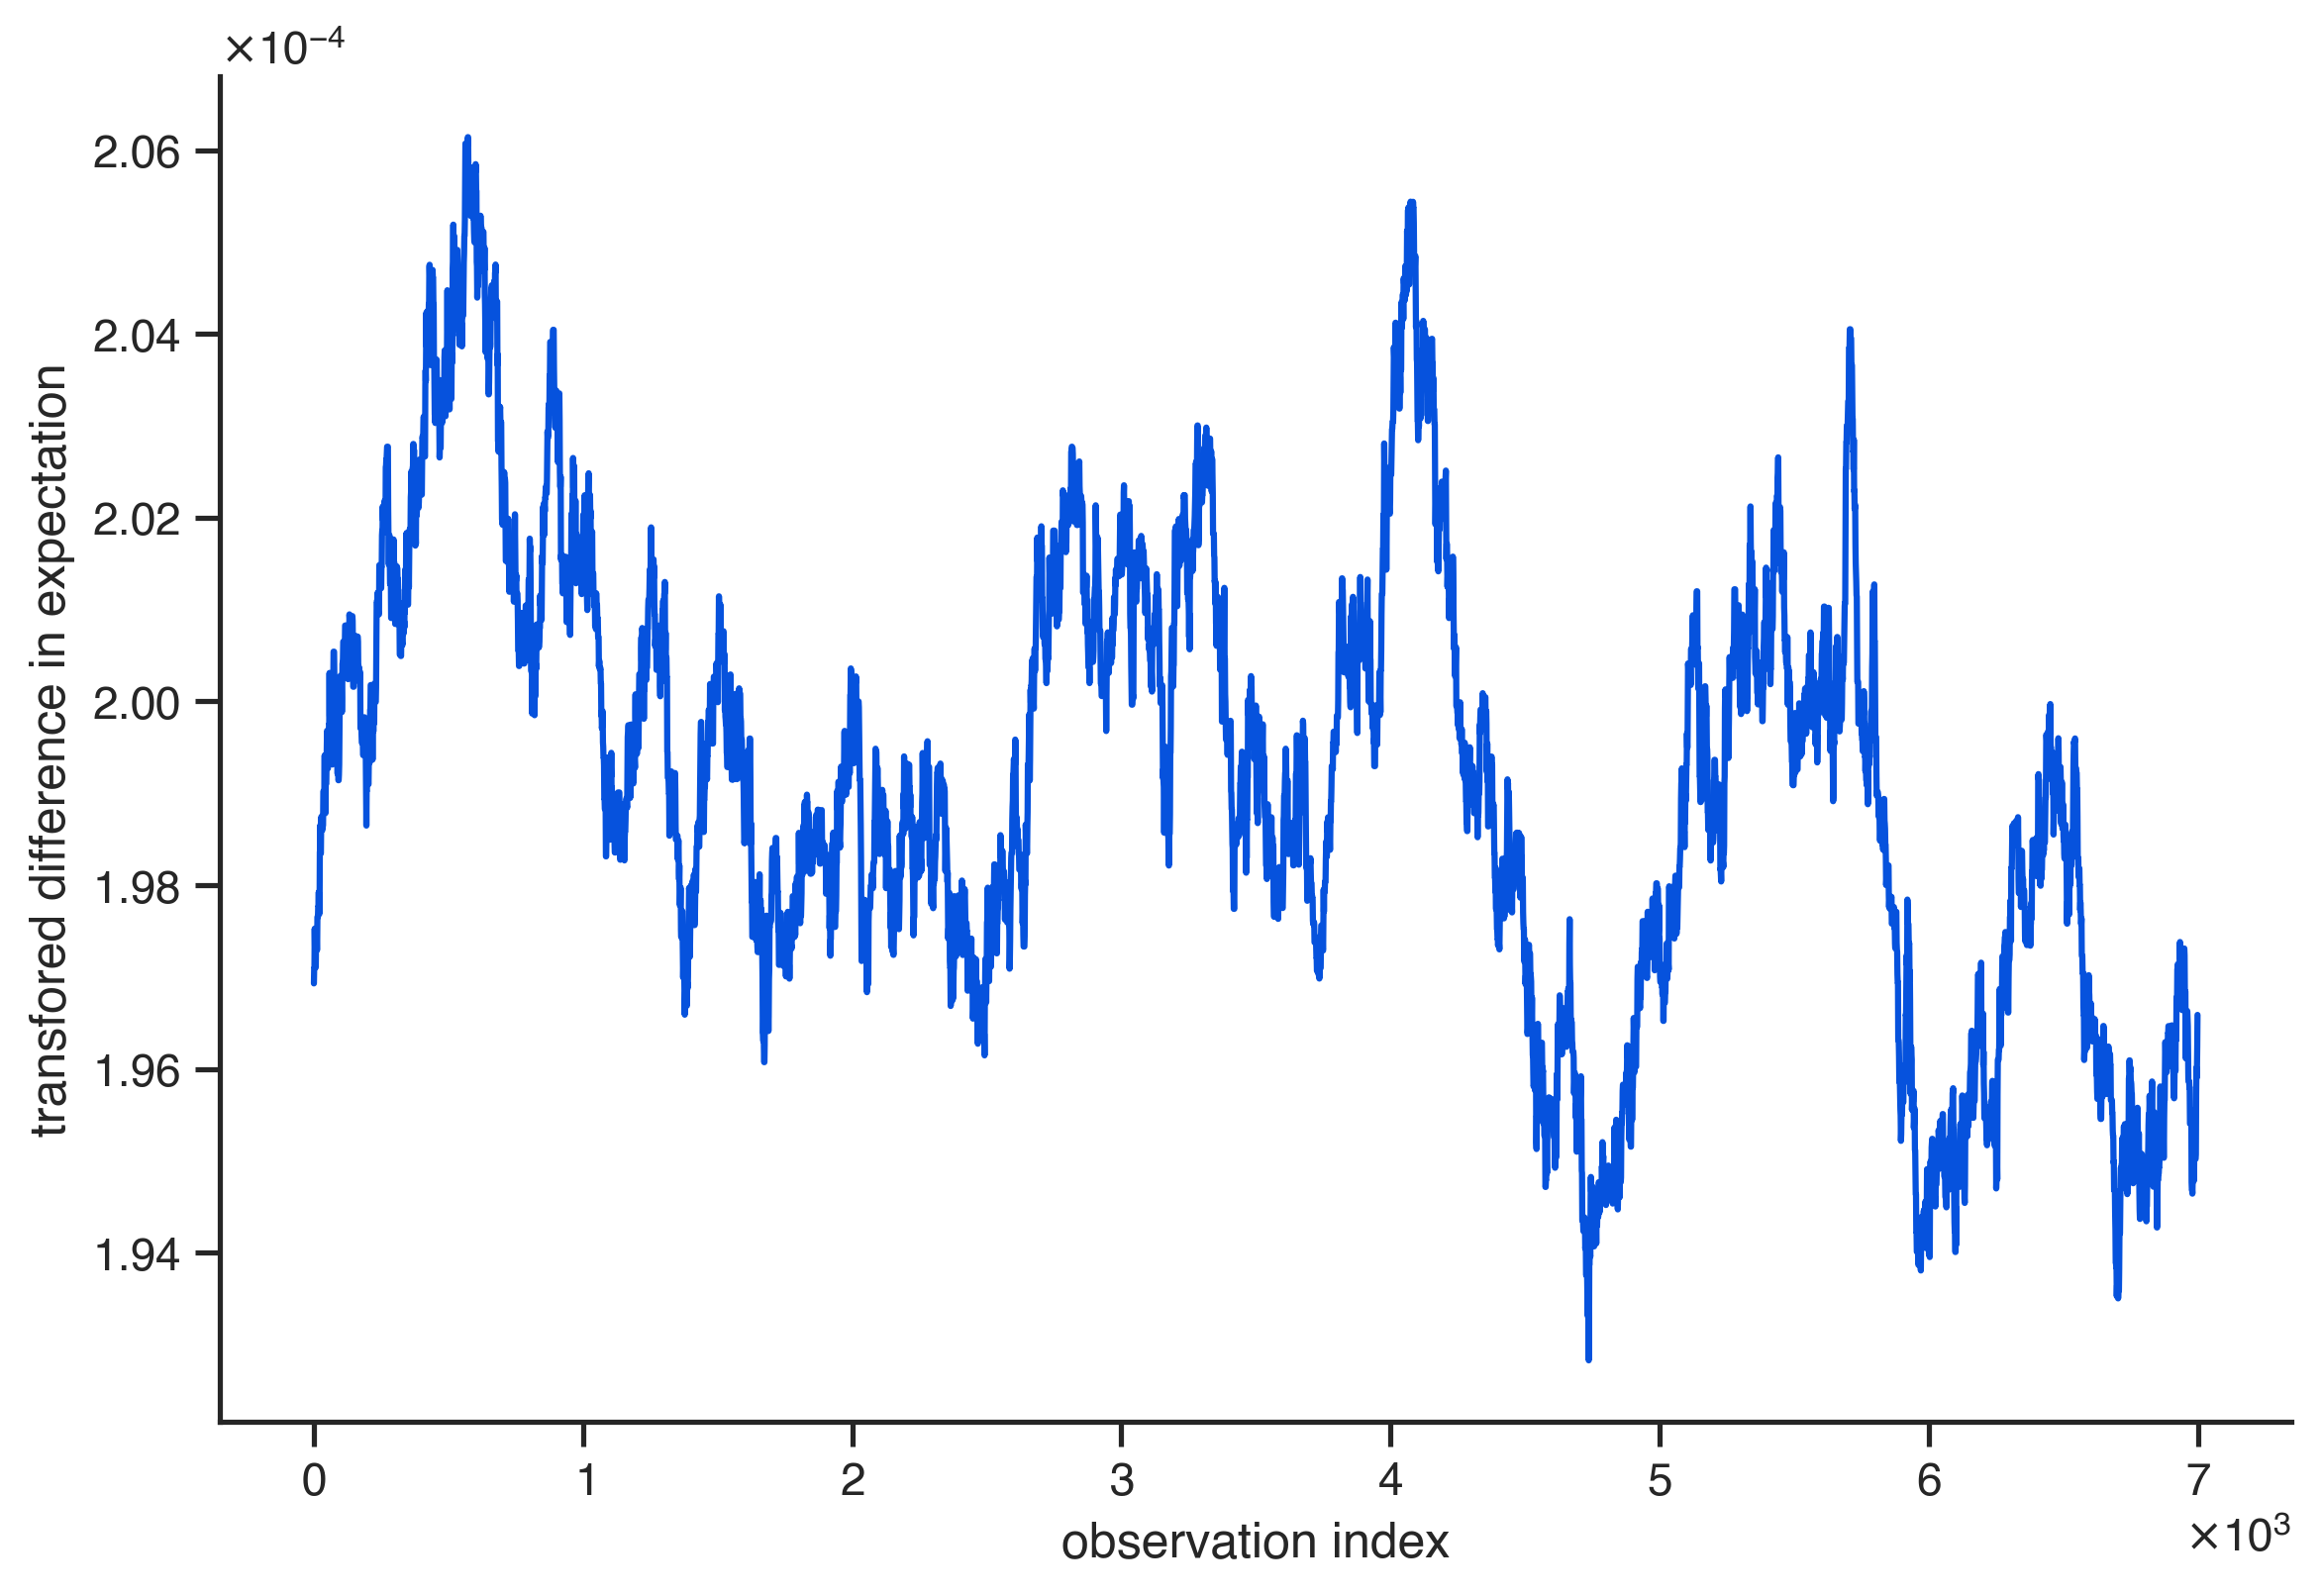
\includegraphics[width=\linewidth]{figures/cm_2015_ward_trace_plot.png}
 \caption{A Trace of the Sigmoid Difference in Expectation of the Probabilistic Hypercubes in the DVM Chain for Chicago's 2015 Mayoral Runoff Election}
 \label{fig:chi_cm_2015_trace}
\end{figure}

\begin{figure}[ht]\centering
 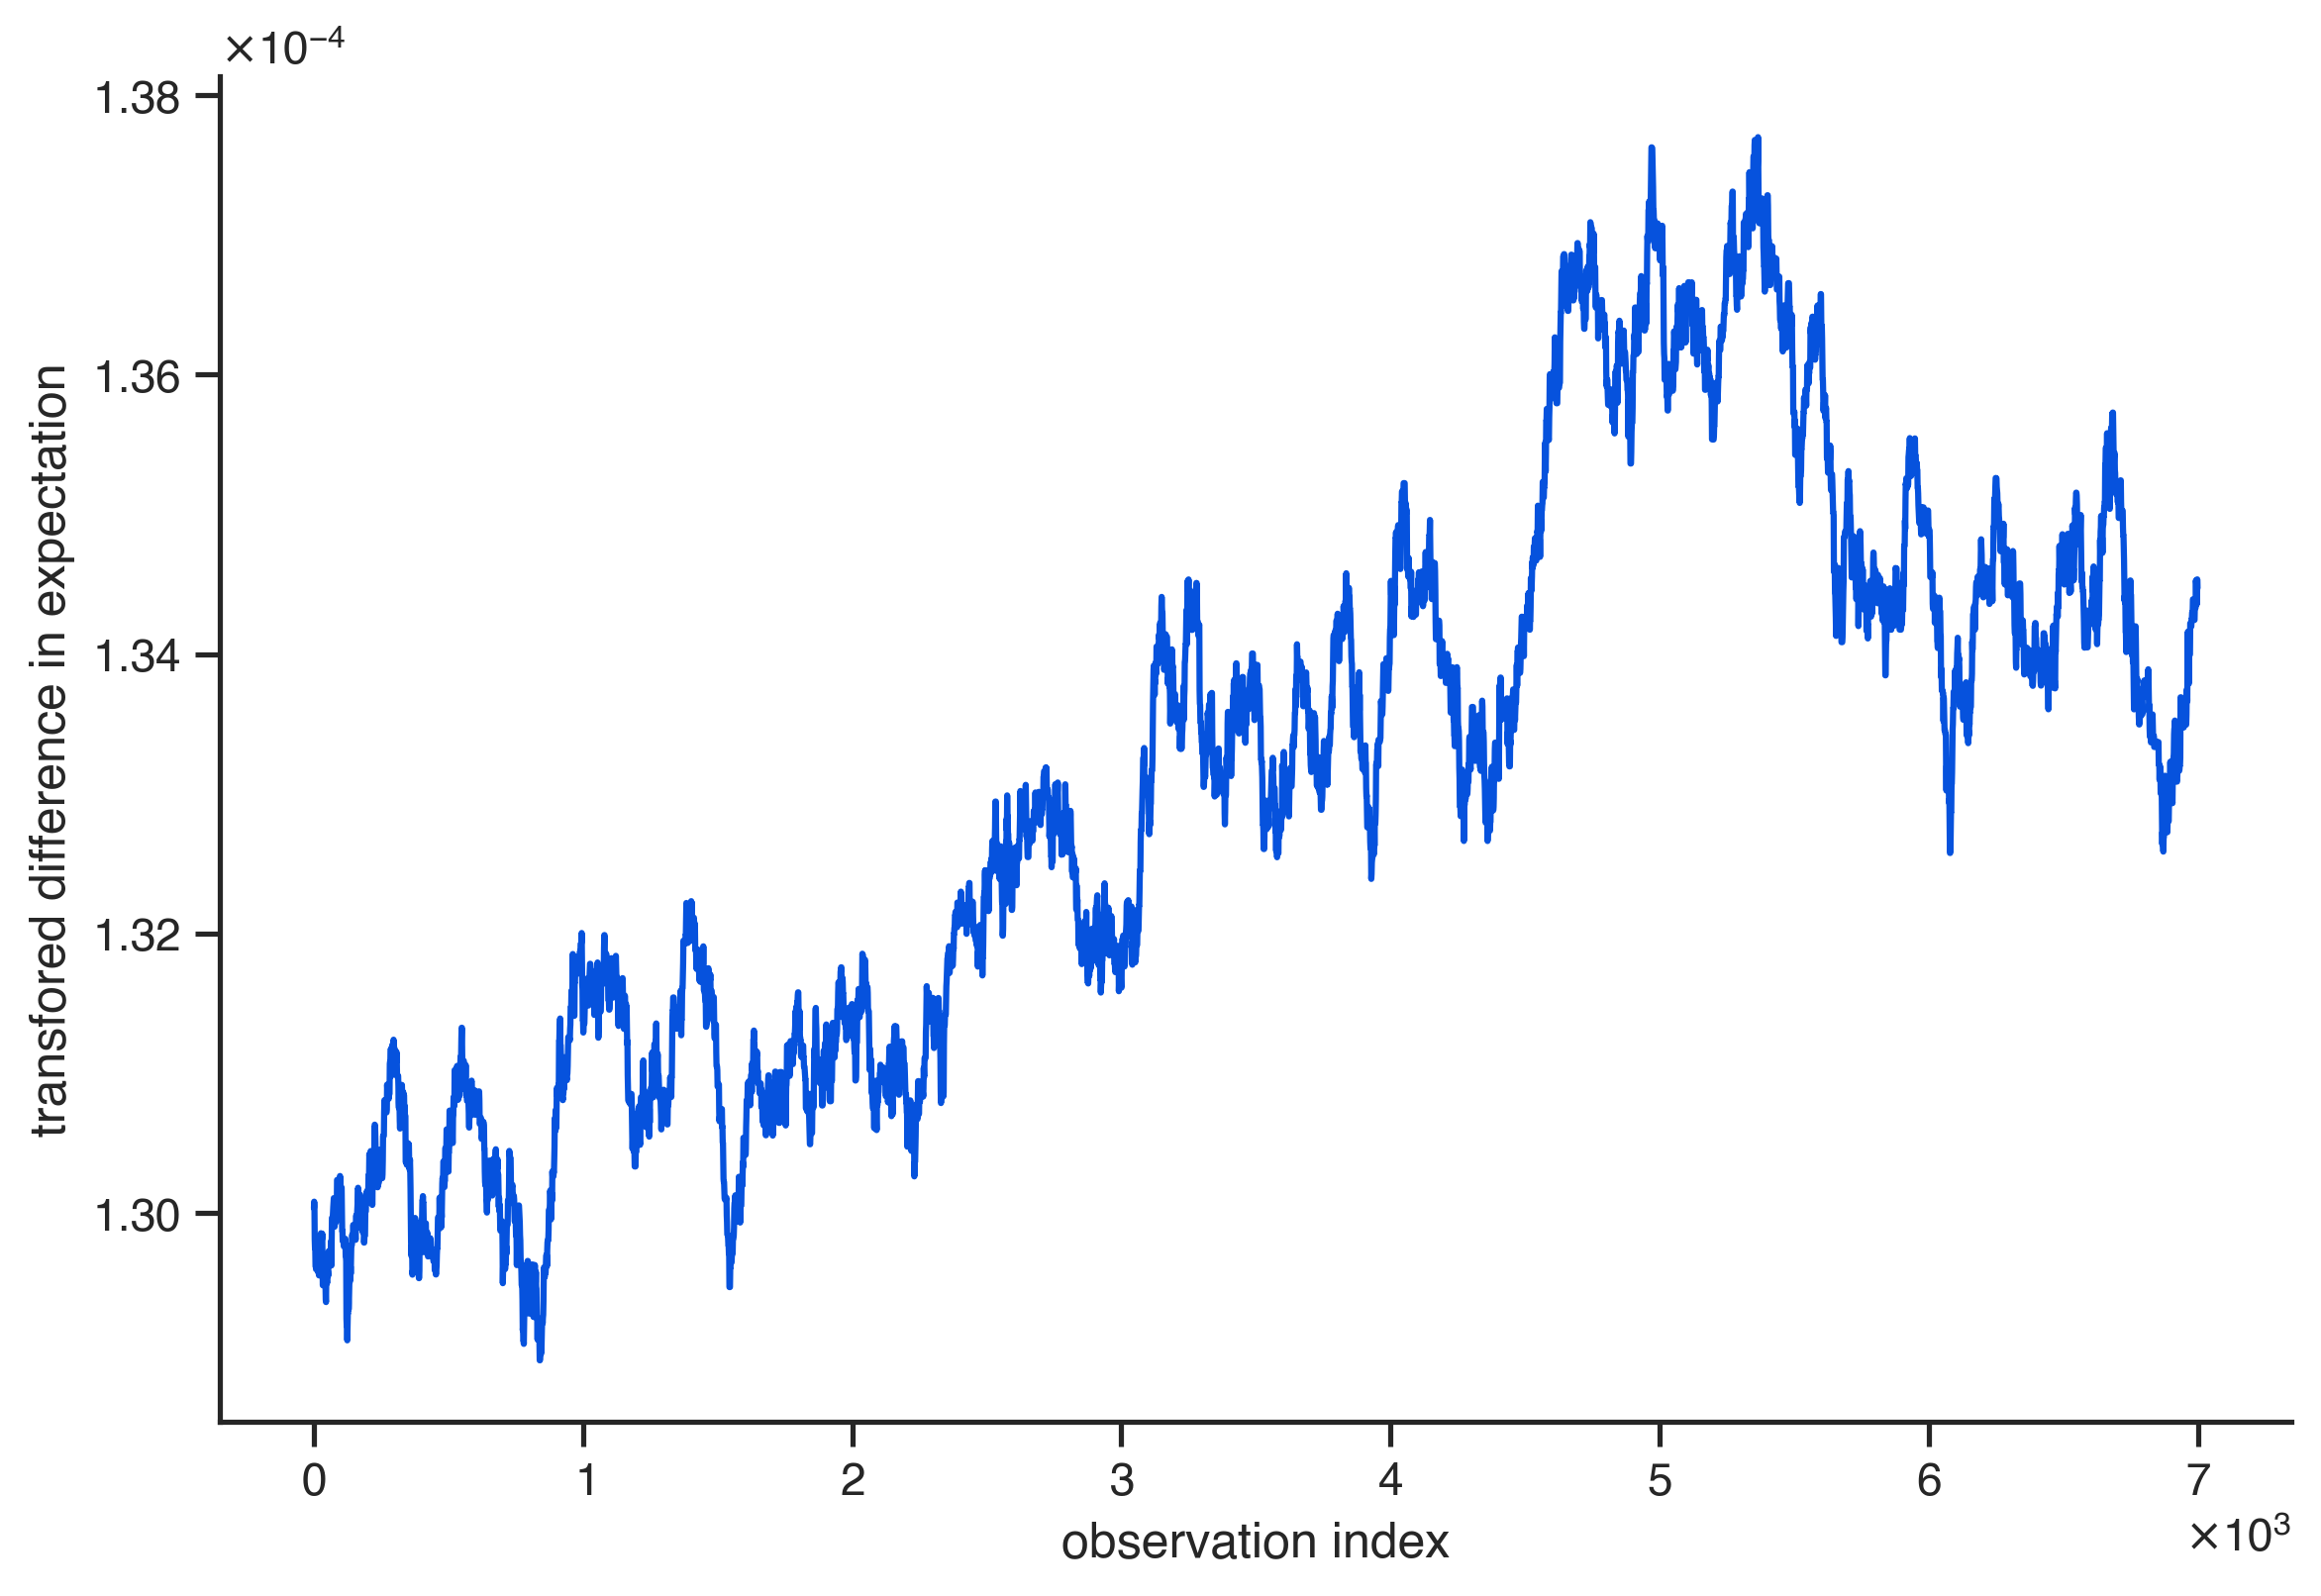
\includegraphics[width=\linewidth]{figures/cm_2019_ward_trace_plot.png}
 \caption{A Trace of the Sigmoid Difference in Expectation of the Probabilistic Hypercubes in the DVM Chain for Chicago's 2019 Mayoral Runoff Election}
 \label{fig:chi_cm_2019_trace}
\end{figure}

\begin{figure}[ht]\centering
 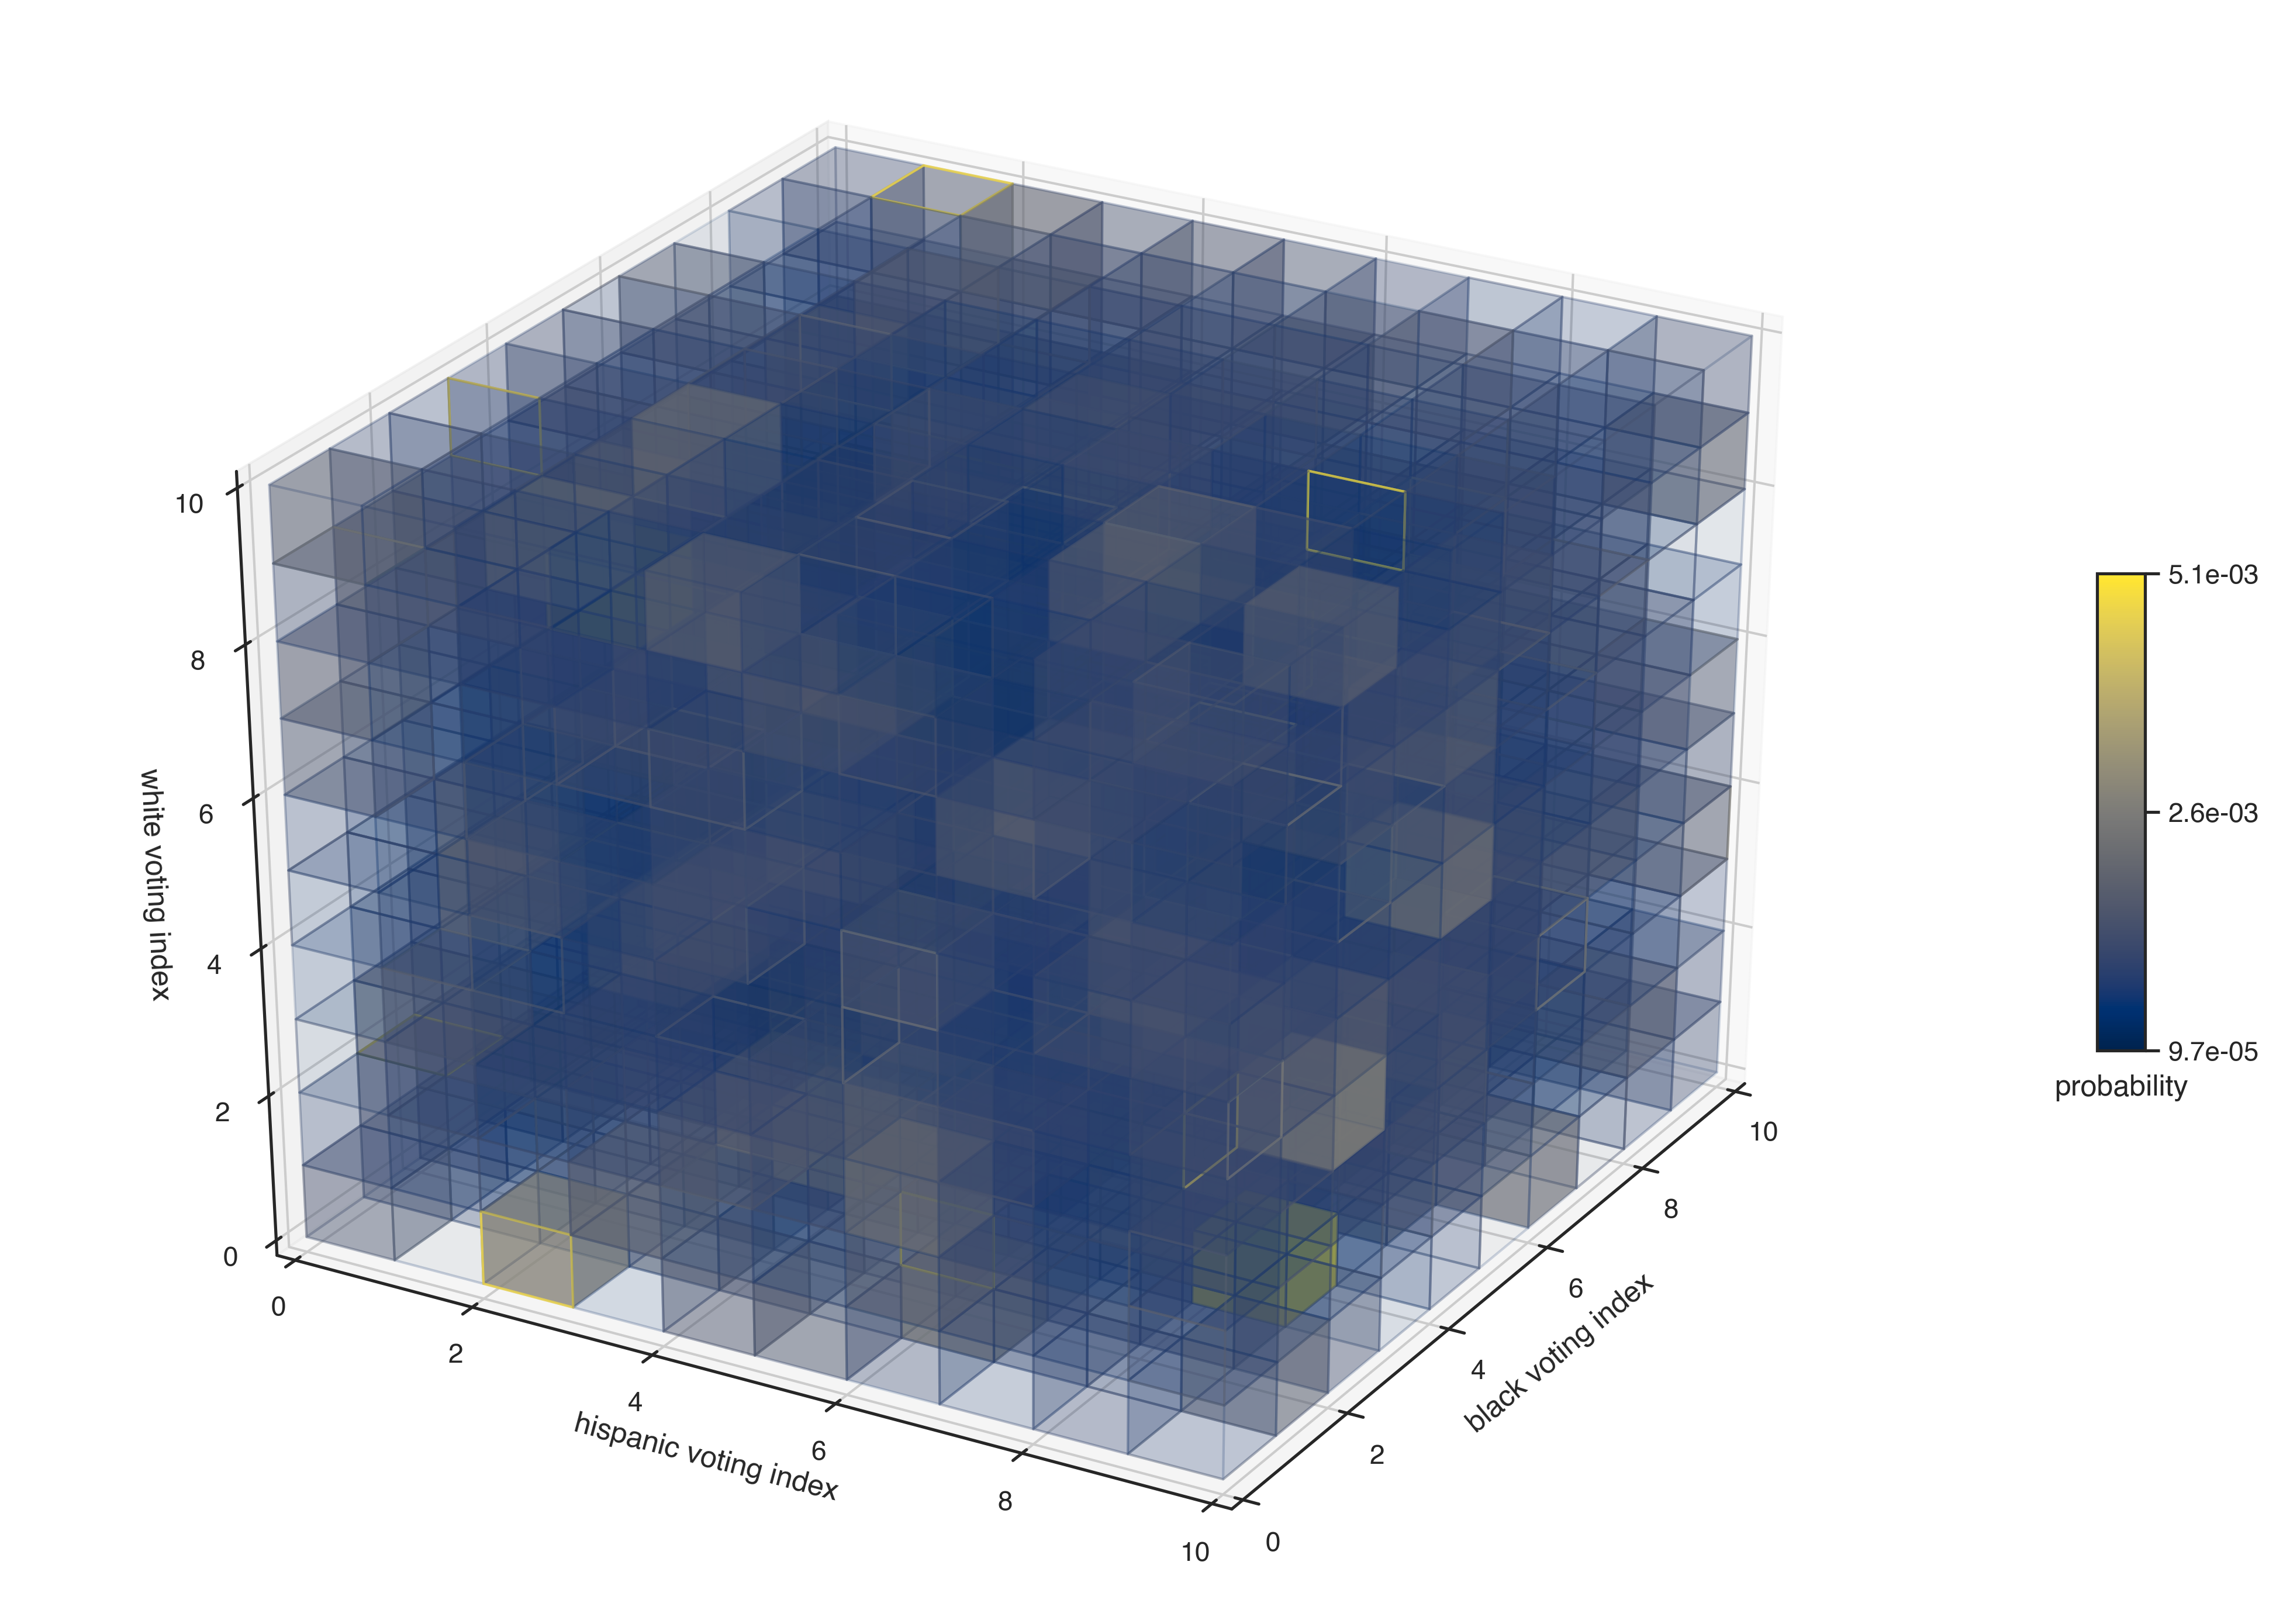
\includegraphics[width=\linewidth]{figures/cm_2015_mean_phc.png}
 \caption{The Mean PHC for the 2015 Chicago Mayoral Runoff, for Rahm Emanuel}
 \label{fig:cm_2015_mean_phc}
\end{figure}

\begin{figure}[ht]\centering
 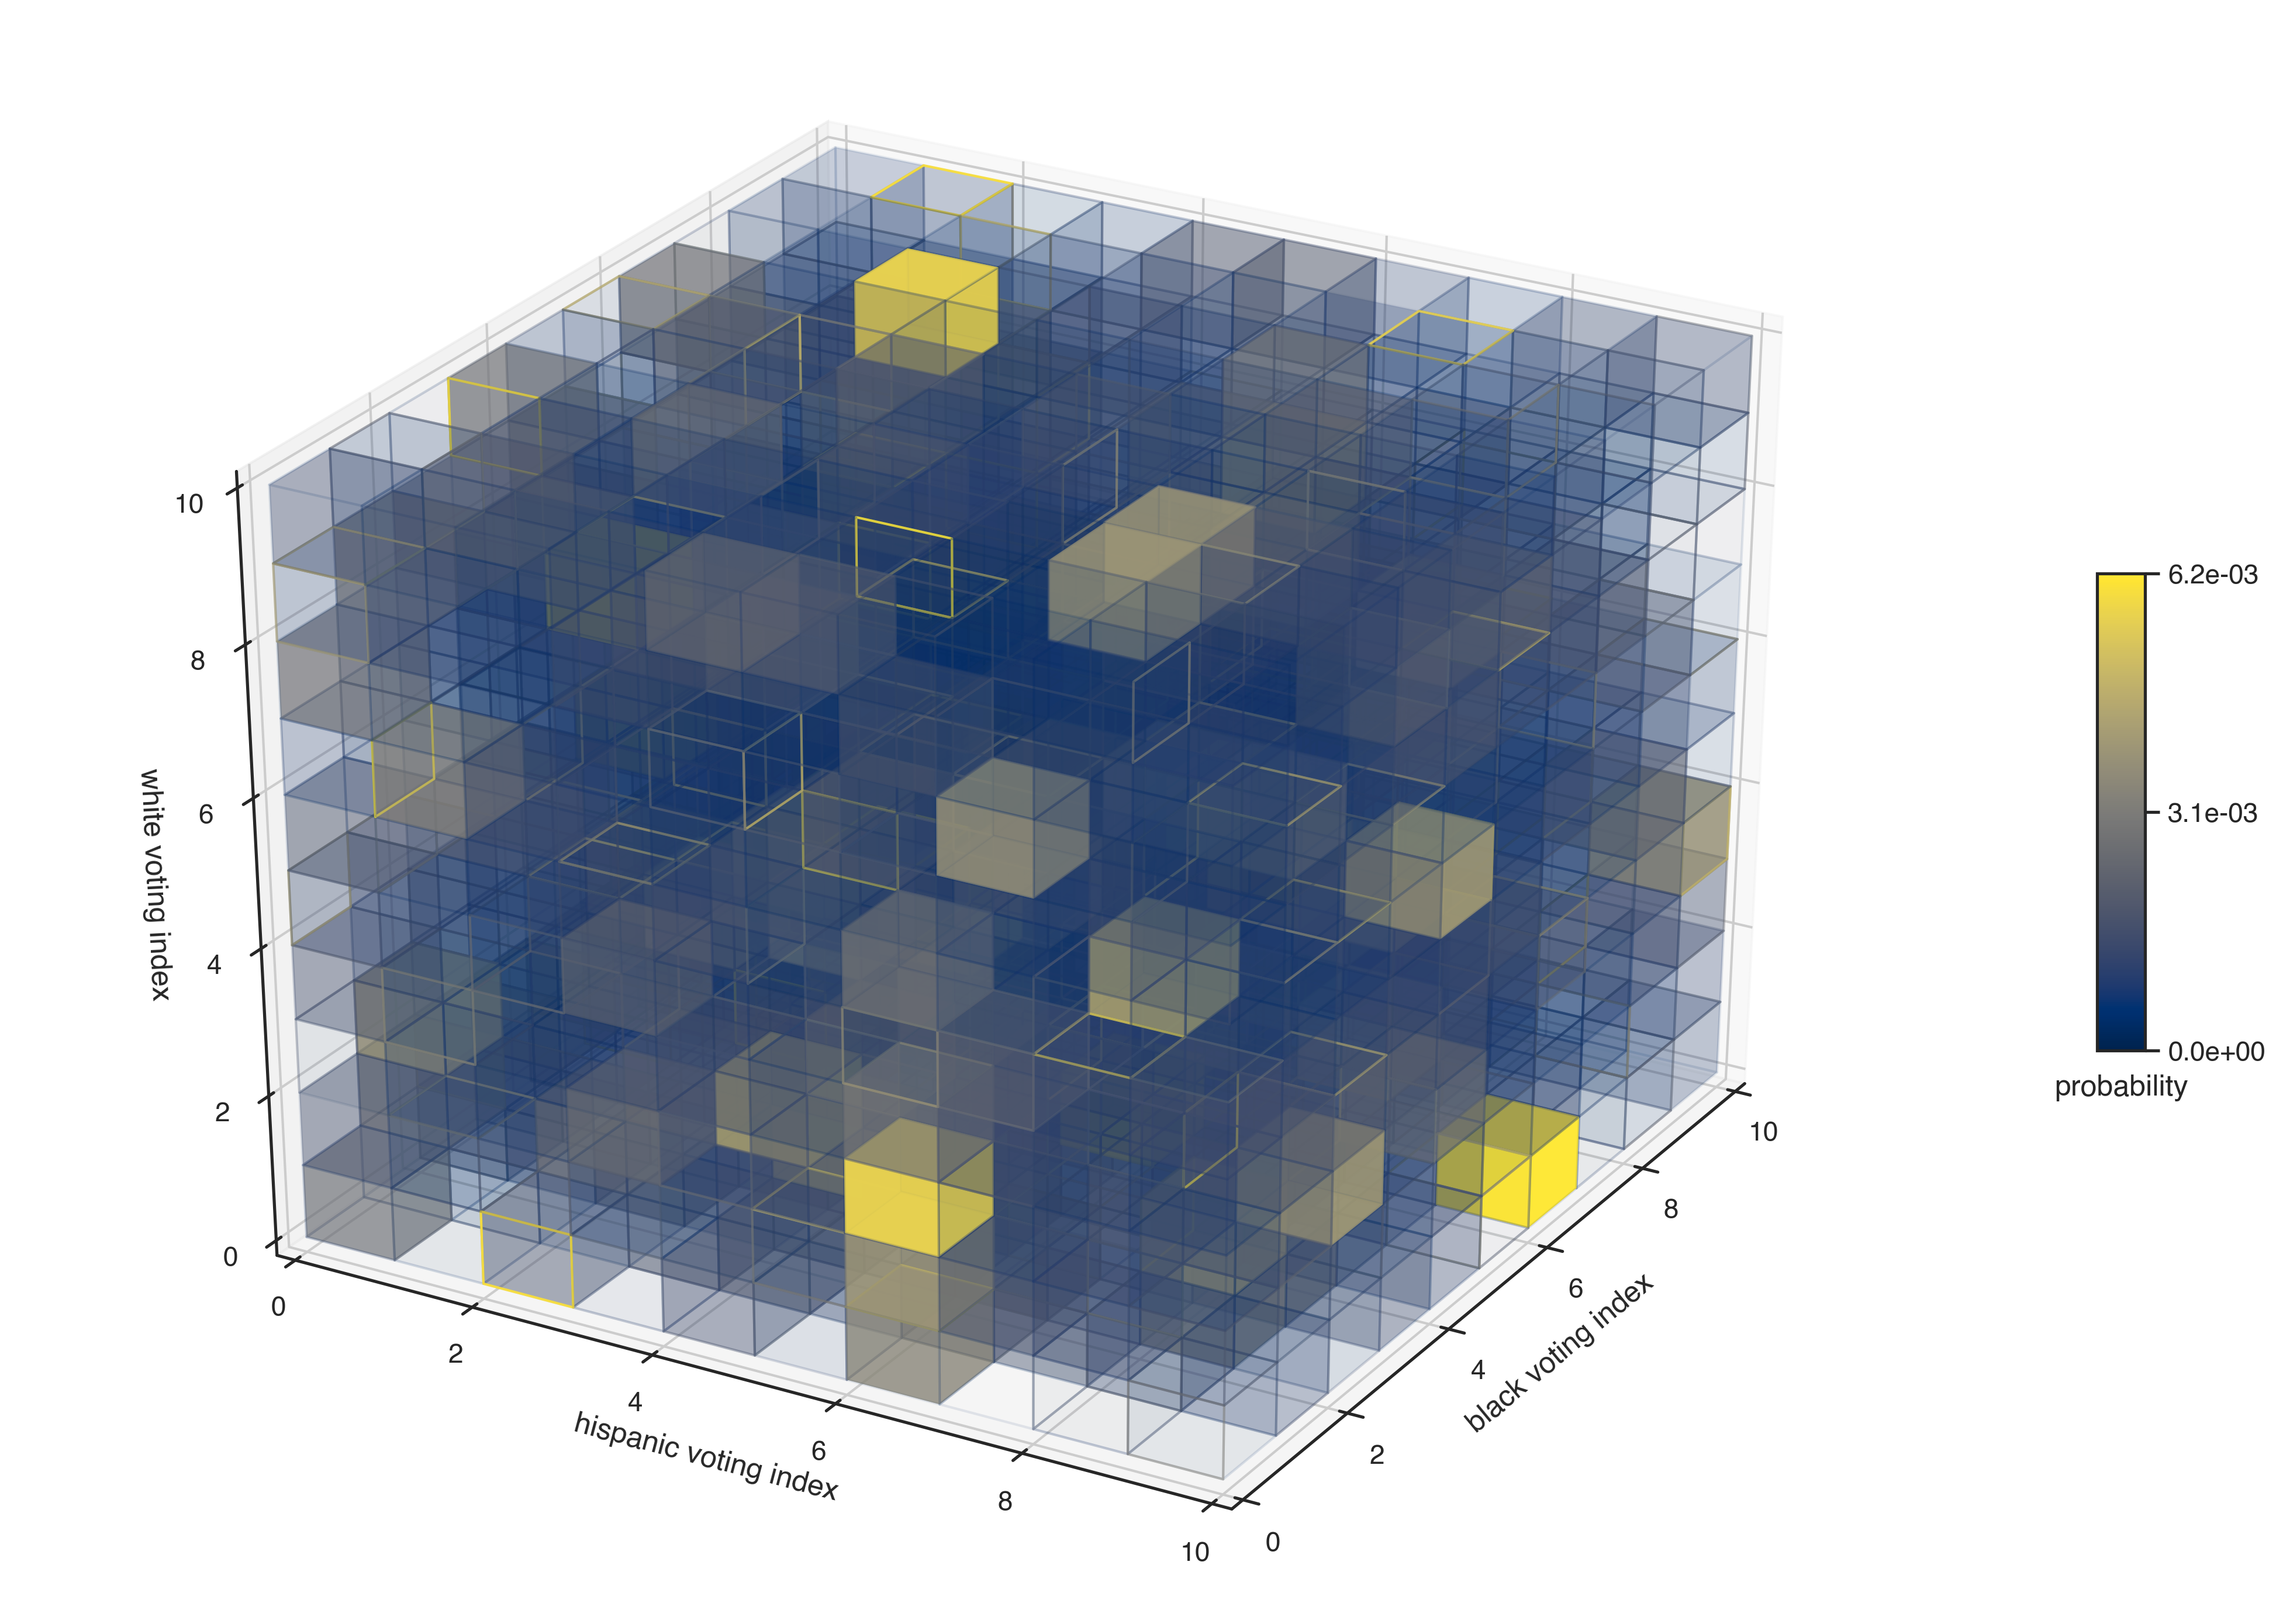
\includegraphics[width=\linewidth]{figures/cm_2015_mle_phc.png}
 \caption{The MLE for the 2015 Chicago Mayoral Runoff, for Rahm Emanuel}
 \label{fig:cm_2015_mle_phc}
\end{figure}

\begin{figure}[ht]\centering
 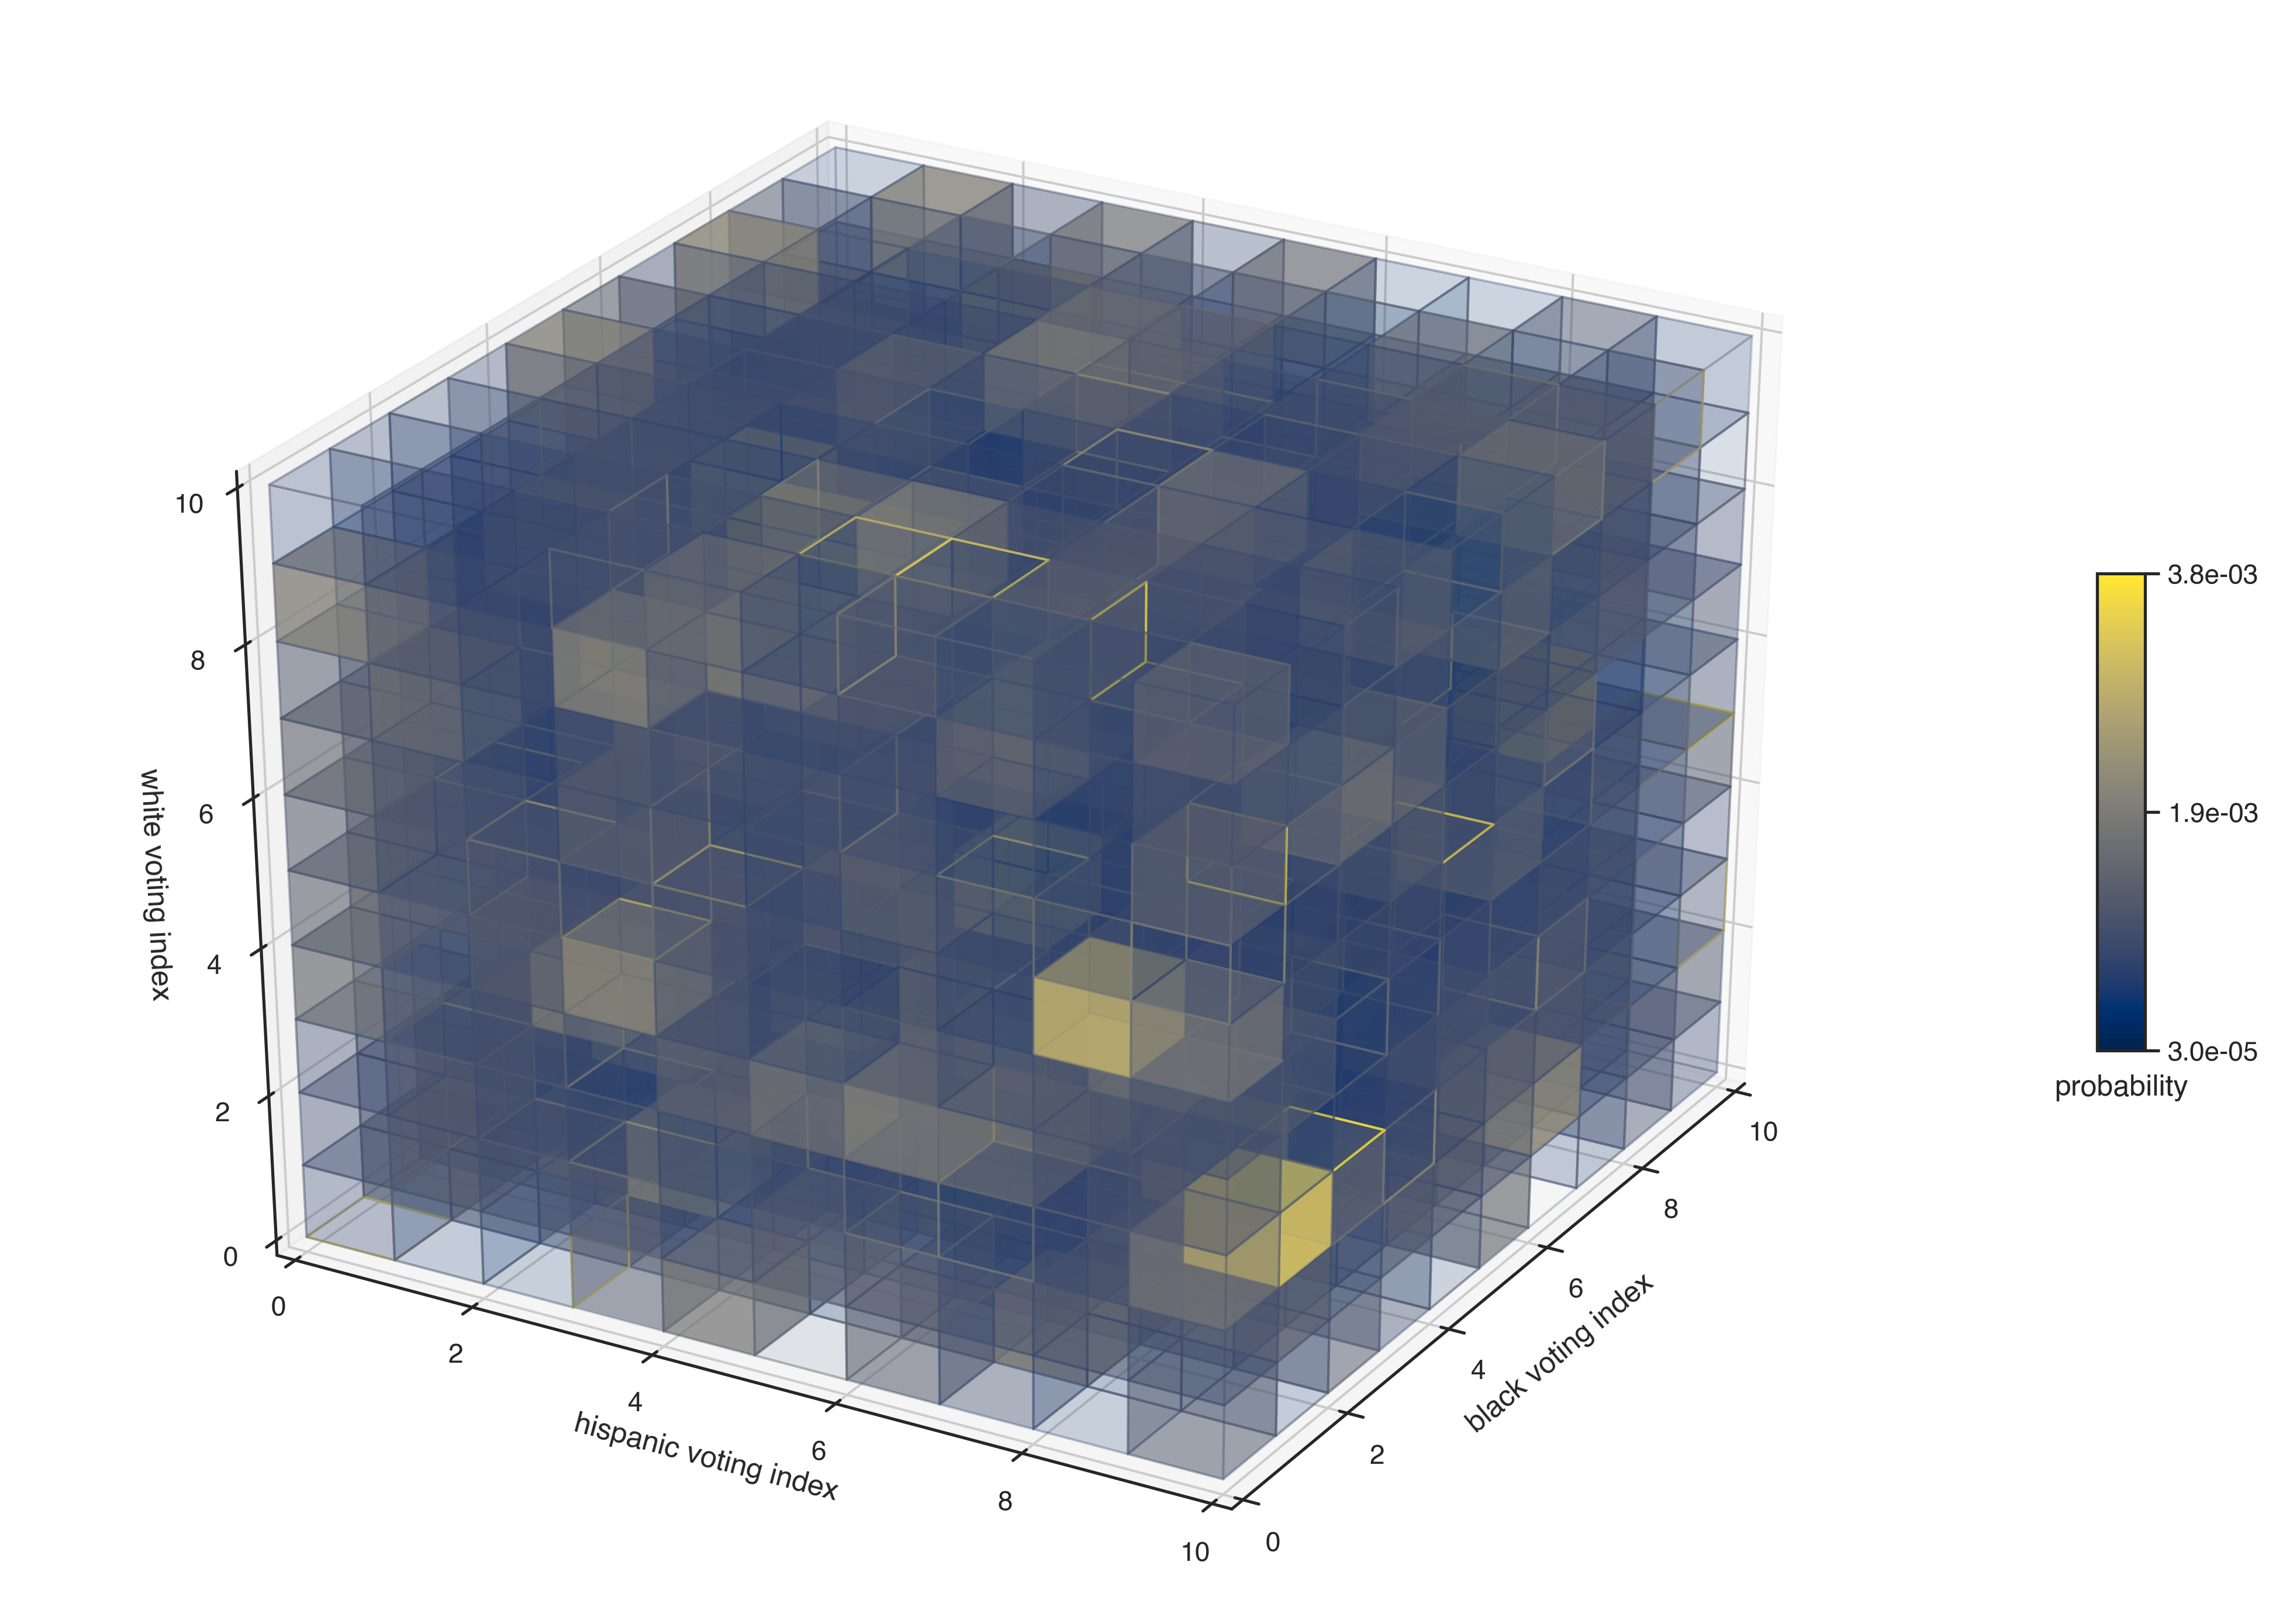
\includegraphics[width=\linewidth]{figures/cm_2019_mean_phc.png}
 \caption{The Mean PHC for the 2019 Chicago Mayoral Runoff, for Lori Lightfoot}
 \label{fig:cm_2019_mean_phc}
\end{figure}

\begin{figure}[ht]\centering
 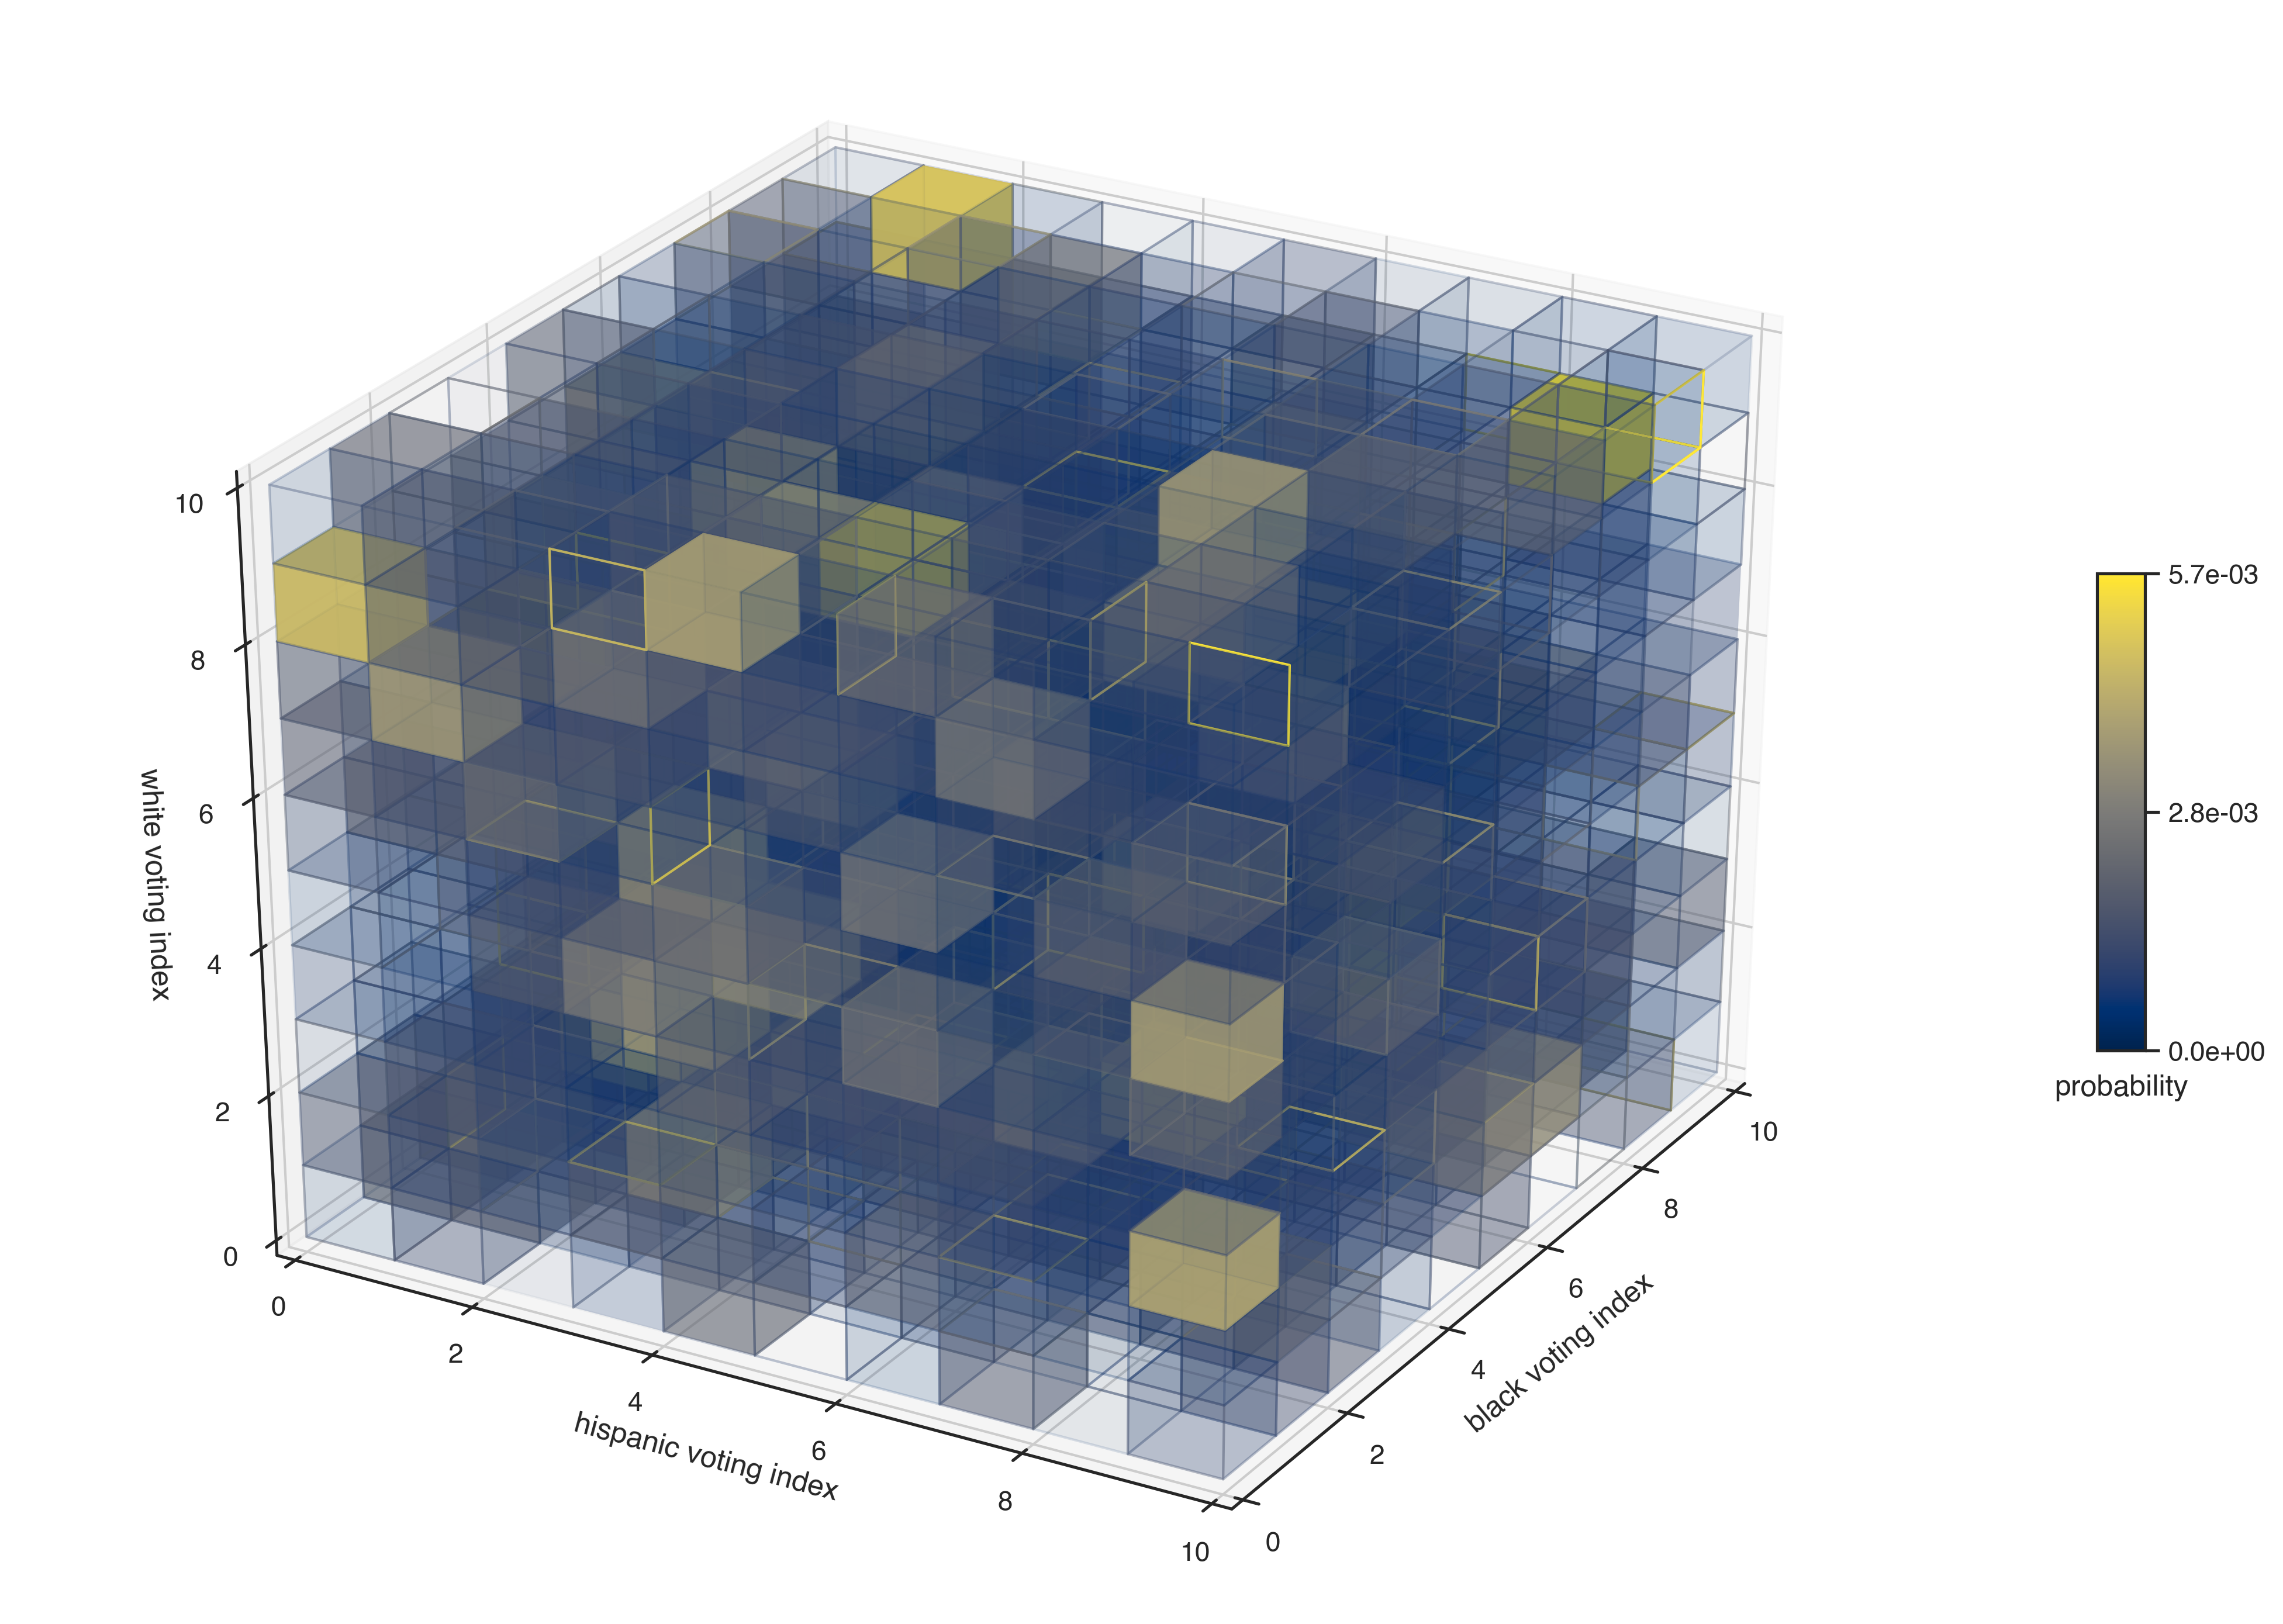
\includegraphics[width=\linewidth]{figures/cm_2019_mle_phc.png}
 \caption{The MLE for the 2019 Chicago Mayoral Runoff, for Lori Lightfoot}
 \label{fig:cm_2019_mle_phc}
\end{figure}

Figures \ref{fig:chi_cm_2015_trace} and \ref{fig:chi_cm_2019_trace} show the trace plots of the Markov chain. The higher the point on the $y$ axis, the more likely the probabilistic hypercube at that state was to have been able to generate the outcome of the election. A trace plot of a well-mixed and converged Markov chain oscillates a bit, then plateaus near the end of the sample. Neither of these trace plots show particularly poor behavior, but it is not clear that the chain has converged, or is close to convergence, either.

Figures \ref{fig:cm_2015_mean_phc} to \ref{fig:cm_2019_mle_phc} illustrate the mean and MLE probabilistic hypercubes for the sample generated by DVM. They are all quite intuitive in their suggestions. In neither election is much probability concentrated at the edges of the PHC. If that were the case, there would be massive amounts of racially polarized voting. Instead, the PHCs show some probability concentrated at the edges, with most of it toward the center.

The concentration of probability at the edges suggests that there is at least some racial voting polarization, but that it is not unreasonably dominant. For example, Figure \ref{fig:cm_2019_mean_phc}, the mean PHC for Lori Lightfoot in the 2019 Chicago Mayoral runoff election, shows that there is a relatively high probability that she was quite popular with Hispanic and Black voters, which does match anecdotal evidence.\cite{negocios}.

These probabilistic hypercubes can then be used with precinct data to choose some demographic voting probability. For example, using the PHC represented in \ref{cm_2019_mean_phc}, one can supply a ward, say ward $1$, and find that a likely set of demographic voting probabilities for that ward is that $\approx 90\%$ of Black voters,$\approx 55\%$ of Hispanic voters, and $\approx 25\%$ of white voters preferred Lori Lightfoot over Toni Preckwinkle. Those numbers, inferred with the Discrete Voter Model, are the unknowns in the ecological inference problem. Black and Hispanic voters seem to prefer this candidate, so there is some racial voting polarization. While these results are the outcome of a probabilistic process, and thus inherently non-deterministic, the experiment and case study are quite repeatable. Not only do they yield similar results, but they also yield similar probability hypercube distributions. The PHC object can thus express more about the Chicagoan electoral landscape than ever before.


\section{Implications}

\newthought{The strength of the Discrete Voter Model} is its ability to represent the complex voting relationships between and within demographic groups, no matter how many groups there are. The only limitation is time and computing power, but DVM is already written such that it can be easily scaled to more powerful modern architectures. The rise of cloud computing, and particularly infrastructure as a service (IaaS) products like Google Compute Engine and AWS EC2, allows for the relatively inexpensive rental of unprecedented computing power. The experiments in Chapter \ref{chap:results} and the case study in Section \ref{sec:chicago} were run on a typical laptop computer, and they were still able to produce good results.

The Discrete Voter Model's flexibility will allow for the analysis of how a bevy of important aspects of voters' identities and experiences affect their ability to vote and that vote's power in elections. While race is unfortunately a critically important determinant of one's political power, other characteristics, like age and income, may also affect that power. Since the ``demographic group" is abstract, it can be easily replaced to analyze these other characteristics. DVM not only scales with the number demographic groups, but also the size of the election. Hence, these methods can be applied to cities like Chicago, and states like North Carolina without changing the statistical foundation or the implementation.


\section{Future Work}

\newthought{The Discrete Voter Model} will continue to be evaluated on more complex elections, for longer runs, and on more powerful computing infrastructure. It will also be continually maintained and improved. Options for future work include:

\begin{enumerate}
  \item adding more transition kernel options
  \item adding more scoring function options
  \item translating the model's execution phase to a more numerically-performant language, like C++
  \item exploring other shapes for probabilistic hypercubes. Promising alternatives include making the $n$ dimensions more abstract, and working only with flat tensors to improve performance.
\end{enumerate}
